\chapter{Metodologia}
\label{cap:03}
A metodologia para alcançar os resultados do estudo comparativos, será dividido em 4 etapas,
 na figura~\ref{fig:diagramaMetodologia} abaixo elas são:

\FloatBarrier
\begin{figure}[!htbp]
	\centering
	\caption{Diagrama da metodologia do estudo comparativo}
	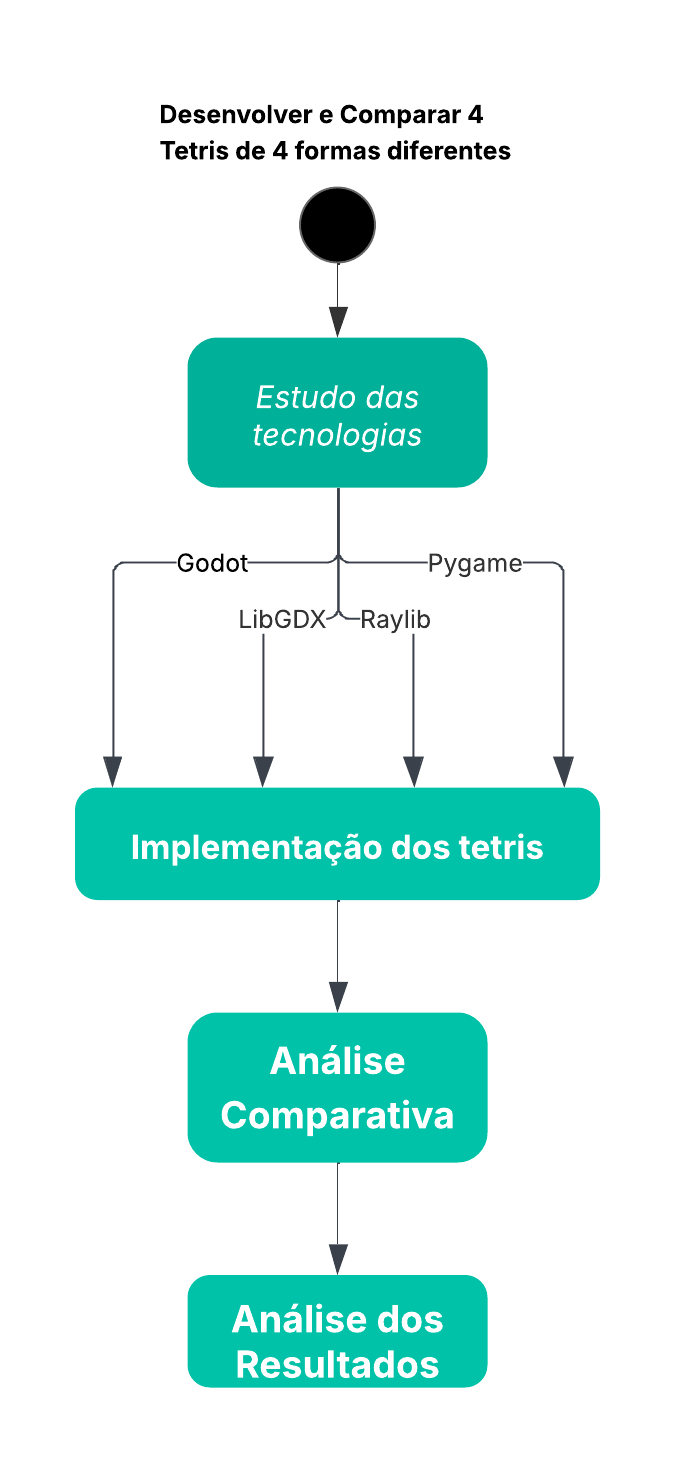
\includegraphics[scale=1.2]{imagens/DiagramaMetodologia.png}
	\\\textbf{Fonte:} Feito pelo autor
    \label{fig:diagramaMetodologia}
\end{figure}
\FloatBarrier
\subsection{Estudos das Tecnologias}

    Para cada linguagem de programação e sua respectiva \textit{engine} e seus respectivos \textit{frameworks} (\textit{Godot}, Pygame, Raylib, LibGDX)
    será feito um estudo inicial para aprender como funciona a estrutura de cada \textit{framework} e seus principais métodos, 
    o ciclo de vida de um jogo tanto da \textit{engine} como nos \textit{framework} é praticamente igual, com algumas diferenças entre si, o que
    tornará o processo de aprendizagem menos complexo. O estudo será feito de forma prática, consultando documentações oficiais e materias complementares conforme a necessidade do desenvolvimento, 
    a etapa do estudo das tecnologias e a implementação ocorrerá paralelamente.

\subsection{Implementação dos \textit{Tetris}}
    O \textit{Tetris} pode ser categorizado como um jogo de quebra-cabeça, em uma grade 10 colunas por 20 linhas, 
    o jogador empilha formas geometricas denominadas \textit{tetrominós},
    assim que uma linha inteira é preenchida, essa linha é retirada e as outras serão deslocadas para baixo, 
    assim liberando espaço para a continuidade do jogo \cite{TetrisWin}, os \textit{tetraminós} são formas geometricas composta sempre por 4 quadrados,
    há 7 \textit{tetraminós} que o jogador pode controlar, são eles mostrado na figura~\ref{fig:tetraminoes} abaixo:

    \FloatBarrier
\begin{figure}[!htbp]
	\centering
	\caption{Os 7 \textit{tetraminós}}
	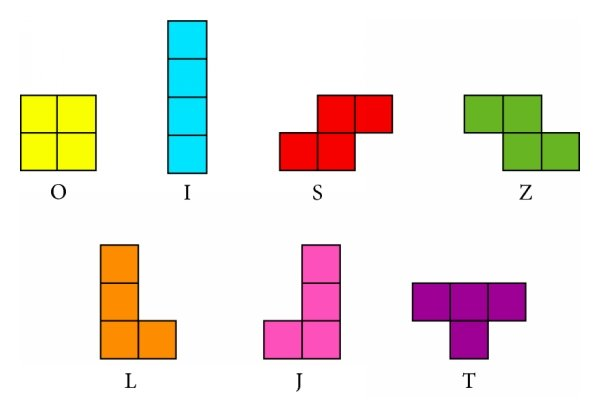
\includegraphics[scale=2]{imagens/tetraminoes.png}
	\\\textbf{Fonte:} \cite{networkTetris}
    \label{fig:tetraminoes}
\end{figure}
\FloatBarrier

     O objetivo do jogador é evitar que a pilha de peças chegue até o topo da grade, conseguindo jogar pelo maior tempo possível \cite{TetrisWin}.
    A escolha do jogo \textit{Tetris} para implementação e comparação foi por que é um jogo clássico 
    de lógica simplificada, porém necessita recursos fundamentais que uma ferramenta de desenvolvimento 
    de jogo oferece como por exemplo: renderização gráfica, detecção de colisão, manipulação de array de duas
    dimensões, controle do jogador, atualização de telas e outros recursos.
    Será feita a implementação do jogo 4 vezes:
    \begin{itemize}
        \item Implementação em \textit{Godot};
        \item Implementação em Java utilizando a ferramenta \textit{LibGDX};
        \item Implementação em C++ utilizando a biblioteca \textit{Raylib};
        \item Implementação em Python utilizando a biblioteca \textit{Pygame}.
    \end{itemize}

\subsection{Análise comparativas}

Após a implementação dos \textit{Tetris} será avaliado o tempo de desenvolvimento em cada tecnologia usada,
junto da avaliação da curva de aprendizado e nível de dificuldade, se a tecnologia tem recursos e funcionalidades que facilitam o desenvolvimento,
também será avaliado qual o consumo de CPU em cada um dos jogos executados, consumo de memória RAM e performance em geral.

\subsection{Resultado das análise}

A partir dos dados obtidos da análise, será discutido as vantagens e as desvantagens de cada tecnologia, 
e qual tecnologia apresenta maior adequação para diferentes perfis de desenvolvedores, iniciantes ou avançados.

